\chapter{Introduction}
\thispagestyle{empty}
\label{ch:intro}
\newpage
\refsection

This dissertation consists of a collection of publications and proposes several
methods with which to facilitate the retrodigitization of historical
Arabic-script material. While we are only concerned with the Arabic script
here, our findings are relevant to the analysis of writings and inscriptions in
other writing systems.

\section{Document Image Analysis and Optical Character Recognition}
\sectionmark{Document Image Analysis}

Document Image Analysis (DIA) is a subfield of Computer Vision (CV). It aims at
understanding document content through the processing of its associated digital
images. The term “document” is defined loosely as including both handwritten
and printed text on paper, as well as writing on other supple supports (e.g.
papyrus and palm leafs) or even inscriptions.

Rather than the methods employed, it is the nature of the input images that
differentiates Document Image Analysis (DIA) from other fields in Computer
Vision (CV).  These images are usually obtained through cameras or scanners,
often in a professional setting, resulting in source material with minimal
noise from non-pertinent elements which are often encountered in the natural
scene images treated by other branches of CV.  Notwithstanding the cleaner
input data, the structured representations desired as output tend to be of
higher complexity and quantity in DIA than other applications, requiring
detection, classification, and relation of dozens to hundreds of document
elements such as lines, characters, illustrations, and tables. 

Like other fields of computer science, DIA research can be subdivided into
particular tasks, and specific and targeted methods are designed to solve one
or more of them. The most prominent task in DIA research is optical character
recognition (OCR)\footnote{While in most contexts optical character recognition
and handwritten text recognition are treated as distinct, both are subsumed
under the term OCR here. A detailed justification is given in \ref{s:soa}},
although other tasks also exist, whether they be based on OCR or entirely novel
(e.g. document classification and dating, or keyword spotting).

OCR is the conversion of printed, written, or inscribed writing into
machine-encoded text. It is a well-established process, both as a task in
computer vision research as well as for practical day-to-day applications,
ranging from address parsing to aids for the blind. As a matter of fact, it is
the latter which motivated the first and earliest attempt at creating a
document image analysis system, with an 1809 US patent for a non-tactile
reading instrument. Early systems were rudimentary and their output required
significant human interpretation. Fournier D’Albe’s 1914 optophone, for
instance, converted strokes into tones and expected the reader to interpret
them mentally as character information. Such systems were little more than
intellectual curiosities at the time and none of them achieved widespread use.

These early explorations preceded the invention of computers by several
de\-cades. Their evolution into modern-day DIA techniques has allowed for a broad
range of applications in tasks such as address parsing for mail routing, cheque
verification and book retrodigitization. It is now a claim largely unchallenged
in the field that OCR is fundamentally solved at least for modern,
machine-printed documents in English with a reasonable low level of noise, for
which modern commercial retrodigitization software achieve character accuracy
rates above 99\% routinely. Nevertheless, while this holds true for English, we
count almost four-thousand other written languages and several hundred associated
writing systems or scripts. No practical OCR systems are available for the vast
majority of them. Even accounting for the use of purely alphabetic scripts such
as Latin and Cyrillic, which present less of a challenge to state-of-the-art
OCR when employed accordant with modern western typographic practices, it is
clear that a substantial proportion of human literary output is not yet
accessible through retrodigitization.

This is all the more true when we consider historical literary output. While
large scale digital scanning in rich countries has resulted in the creation of
substantial digital libraries, these text are de facto inaccessible to both the
public and scholar, even for material as recent as the late nineteenth century.
Typographical and orthographical variations degrade digitized texts' quality to
a significant extent when transcribed with software geared towards the
treatment of modern documents. For most archival material from the Global
North, this is most likely a temporary situation as projects such as
OCR-D\footnote{\texttt{http://ocr-d.de}} pave the way for greater integration
of pure DIA research into library practice. Other collective and more specific
efforts include \cite{smith2018research}, which gathered both humanities
scholars engaged in digital methods as well as computer vision experts, with
the shared goal of establishing a research program for the digitization of
historical and \emph{minority script} material. Nevertheless, these communities
of interest remain fractured along geographical, linguistic, and professional
boundaries.

Meanwhile, the threat of permanent loss of cultural heritage looms over
collections, at risk of permanent deterioration due to political unrest and
ill-adapted storage conditions, combined with utter lack of funding and limited
interest from parties other than minority populations and a small number of
scholars. Even famed collections such as the manuscripts of Timbuktu have
barely escaped destruction due to conflict in recent years, and humidity
continues to threaten their integrity very much.

Many writings lack a fundamental technological basis to work with: the Berkeley
Script Encoding Initiative alone lists over a hundred writing systems that
remain to be encoded in Unicode. Circa two-thirds of them are historical and a
substantial remainder is used liturgically. Without a standardized way to
represent them digitally, their retrodigitization and dissemination becomes
infinitely more difficult. A number of these writing systems have substantial
scholarly communities – ranging from Egyptian Hieroglyphs and Demotic,
Cuneiform, to a variety of Chinese scripts. Even scripts already encoded in
Unicode often lack code points for certain surface forms required for
paleographic or epigraphic practice. This is not always an oversight. Rather,
it can be the result of the Unicode Consortium’s encoding guidelines which
largely proscribe inclusion of new allographs and ligatures in the standard.
While alternative standards exist (e.g. the code tables as defined by the
Medieval Unicode Font Initiative \footnote{http://mufi.info}), this situation
favors the emergence of ad-hoc standards and thus limits interchangeability and
machine-readability of text considerably.

\subsection{Tasks}

As one of the core applications of document image analysis, OCR has dwelt upon
a large number of its subproblems. Some of them have become obsolete with time,
thanks to the increasing capability of new algorithms. Others are new,
resulting from the need to deal with increasingly challenging material. It is
not necessary to deal with all of them at once to have a functional OCR system.
As a matter of fact, many of them are material-specific, and are of concern
only when dealing with specialized applications. A closer analysis of the
design requirements for a largely script-independent OCR system, capable of
processing Arabic-script text based on a survey of its calligraphic and
typographic features, will follow in chapter~\ref{ch:arabic}.

A non-exhaustive compilation of generally accepted tasks can be found below.

\begin{description}
\item [Binarization] Classifying the pixels of an image into two classes:
foreground, i.e. text, and background, i.e. everything else.
\item [Denoising] Increasing the page image quality for subsequent problems.
Denoising includes processes such as background normalization, color space
adjustments, deblurring, or stain removal.
\item [Deskewing and Dewarping] Correcting both the perspective distortion
inherent in camera capture and other degradations introduced commonly in
scanning setups such as rotation, warping along the binding, \dots
\item [Region Segmentation] Subdividing a page image into components such as text, decoration, notes, \dots
\item [Text Line Segmentation] Extracting the text lines from a page image.
Text line segmentation is notable for being a task where not only a large
variety of techniques exist but the modellisation of the line itself has been
subject to considerable research.
\item [Character Segmentation] Segmenting text on a page image down to the
glyph or even lower level. While a common operation in traditional OCR systems
it is mostly unnecessary with state of the art methods. A related task that is
of interest to the humanities, especially paleo- and epigraphers, is character
alignment, i.e. the locating individual characters on a document page given the
full page text.
\item [Script and Font Recognition] Classifying the language, writing system,
style, or typeface of the text. This classification can be performed at
different levels, such as document-wide or individually for whole or parts of a
line.
\item [Table Recognition] Inferring the logical structure of table images.
\item [Scene Text Recognition] Recognition of text in images taken in the
\emph{wild} that contain substantial non-text content.
\end{description}

To solve these problems, the typical optical character recognition pipeline
uses specific methods, which operate in three distinct steps:

\begin{description}
\item [Preprocessing] Denoising, deskewing and dewarping, and binarization
\item [Layout Analysis] Extracting structural information from document page
images and enriching it with additional semantic information.
\item [Transcription] Extracting textual information from all or a subset of
objects identified by in the layout analysis step.
\end{description}

This characterization holds true for all but the most esoteric pipelines.
However, the exact functional blocks depend heavily on the type and structure
of the documents processed. For example, traditionally, binarization is used as
a simple process to: enable the use of fast binary morphology in the layout
analysis step; reduce the dimensionality of data for classifiers; or, more
generally, as a type of basic feature extractor. The relative ease with which
accurate binarization for high quality scans of machine-printed text on paper
can be computed contrasts with the difficulty of treating documents on other
writing surfaces, faded writing, fragmentation, etc. As a result, methods
geared towards the treatment of the latter kind often attempt to reduce the
reliance on binarization or skip it entirely. Similar to most other
preprocessing steps, there is a tendency today to eliminate binarization
altogether, due to the increased availability of more advanced techniques.
This, however, remains a topic of debate in the research community.

\section{Motivation}

Arabic-script material represents one of the largest literary traditions in
human history, both in terms of volume and geographical spread. Examples range
from religious texts (most prominently the \emph{qurʼān}, the holy book of
Islam) to poetry, and include scientific and legal texts in addition to a large
corpus of administrative records. The sheer number of sources and the diversity
of domains they cover make them a prime target for new paradigms in the
humanities that employ computational methodology, e.g. \emph{distant reading}
and quantitative palaeography. These methods require either large text corpora
or accurate DIA methods based on one or more of the abovementioned component
tasks of an OCR system. As the vast majority of Arabic texts have never existed
in digital form, high quality retrodigitization through OCR favors the
development of a substantial number of Arabic Digital Humanities research
projects.

When I started working on this thesis, humanities scholars working on
Arabic-script texts largely dismissed OCR of machine-printed Arabic text,
especially of historical and multilingual material. This was even true for
scholars already deeply involved in the digital humanities, as well as funding
agencies. At the time, accurate Arabic handwriting recognition was deemed
completely out of reach. A long trail of publications on OCR of simple Arabic
datasets, such as KHATT~\cite{mahmoud2014khatt}, existed and a number of open
and proprietary OCR software (e.g. Tesseract, Abbyy FineReader, Sakhr) did
offer nominal support for the recognition of Arabic-script text.  However, it
never translated into actual scholarly or large-scale library practice. A
multitude of factors accounts for this situation: high error rates caused by
classifiers and segmenters ill-suited to the cursive nature of the writing
system; a lack of readily available software and technical expertise; and
substantial cost and effort required to adapt existing solutions to the
material of interest.

It was soon evident that the challenges that prevented scholars working on
Arabic-script printed and handwritten texts from relying on OCR
mirrored that of many other researchers engaged in retrodigitization of
historical and non-Latin script material. Imitating the prevailing opinion on
Arabic OCR, \cite{widner2017toward} claimed medieval (Latin-script) manuscripts
to be practically impervious to contemporary OCR. Similar statements can be
found elsewhere. This entailed an overall lack of established best practices,
data formats, and requirements on software capability and interfaces suited to
the workflows of digital humanists. Existing projects like
Lace\footnote{\texttt{http://heml.mta.ca/lace/index.html}} and
\cite{alpert2016machine} used OCR technology in an ad-hoc manner. It often
resorted to extensive \emph{data carpentry}\cite{carpentry} and incorporated
significant domain knowledge to boost accuracy to an acceptable level.

Our goal is therefore twofold. While the research presented here incorporates
an understanding of the Arabic writing system and its associated calligraphic
practices, we aim at conceiving a largely script- and language-independent
\emph{universal} OCR system, one that is useful beyond the immediate community
of Arabic-script scholars. It also allows for methods to be evaluated against
non-Arabic datasets when Arabic datasets are not available. As such, if the
algorithms presented here are particularly suitable to Arabic material, it has
been of primary importance in this research to create algorithms that are
universally applicable.

\section{Scientific Contributions}

Most of the work presented here should be read in relation to the broader field
of Digital Humanities. The research presented in the next chapters is not a
heterogeneous collection of methods solving single tasks in DIA that are only
of use to humanities scholars engaged in retrodigitization. It is part of a
coherent ecosystem consisting of two major components: the Kraken OCR engine
and the eScriptorium virtual research environment (VRE). As such, not only does
this research aim at advancing methods for particular tasks; it also seeks to
improve existing scholarly workflows, ones that are more often than not
laborious and impractical to use, not to say completely unworkable.

Kraken is a feature-complete, freely-licensed and modular OCR system. It
differs from other solutions (both open and proprietary) in multiple and
important ways, i.e. target audience, software design, and generalizability.
These differentiated features are the result of its roots as a large-scale
refactorization of the OCRopus source code, that was performed to enable its
integration into a digitization pipeline for scholarly use at the Chair of
Digital Humanities at the University of Leipzig. It boasts a stable application
programming interface and is also highly modular. Users can create their own
workflows or substitute functional blocks with minimal effort. Recognizing the
sheer diversity of OCR systems-related needs among humanities scholars, a
concerted effort has been made to limit implicit assumptions regarding the
functioning of text, and the software accommodates varied material and
transcription guidelines as much as possible. As a result, Kraken performs only
minimal normalization, is fully compatible with Unicode private use area (PUA)
utilization, and supports both horizontal and vertical directions.

A number of case studies were performed as part of the work to enhance Kraken’s
capacity to support Arabic text work. It led to the first detailed analysis of
state-of-the-art OCR methods on machine-printed Arabic text, evaluating their
respective weaknesses and strengths. A first preliminary study was conducted on
a small number of printed classical Arabic-language books, soon followed by a
large-scale retrodigitization feasibility study using a leading Arabic-language
journal published by the American University of Beirut.

Partly as a result of these studies, the engine has been extended in multiple
ways. This thesis contributes two trainable line segmentation systems, a basic
one capable of only detecting baselines, and a more advanced one allowing
region and line segmentation in addition to classification. The latter is
included in Kraken. Initially, a trainable line segmentation method constructed
on top of a U-Net for semantic segmentation was developed. In a second step the
training procedure was adapted to allow joint region and line detection and
inference of line orientation. This second method has also been optimized for
memory usage by employing a ReNet-like stack of separable recurrent layers,
reducing memory consumption by circa fifty per cent in comparison to similarly
performing fully convolutional semantic segmentation networks.

In addition, a basic script and emphasis detection system, built on Kraken’s
text transcription module, was devised.

The segmenter in Kraken is currently the only openly available layout analysis
module in a complete OCR engine which is able to accurately segment complex
curved lines in Arabic manuscripts. In addition, it is the first method
following the baseline paradigm for line modellisation incorporating line
orientation detection. 

A flexible abstraction layer on top of the pytorch neural networking library
has been added which allows the flexible reconfiguration of the artificial
neural networks (ANN) employed for both layout analysis and text transcription
through a lightweight ANN definition language which is able to express many
features of common architectures employed in computer vision tasks (see
appendix~\ref{app:kraken}). This new layer allows the relatively simple addition of
new layer types and thus quick prototyping and efficient hyperparameter
optimization even for endusers without in-depth machine learning knowledge as
has been demonstrated by~\cite{strobel2020much}. 

In contrast to older open engines such as Tesseract and OCRopus which use
custom neural networking backends, a standard library in widespread use in both
industry and the machine learning research community offers a multitude of
benefits such as easier transfer of development skills and automatic or
low-effort inclusion of performance improvements and additional features like
GPU acceleration, distributed training, or model quantization.

\cite[pg. 19]{smith2018research} notes that one of the main obstacles to
advancing OCR for historical and non-Latin texts is lack of training and
evaluation datasets. During the process of putting together the initial case
studies, important efforts were made in this direction. Several thousand lines
of training data for text transcription were annotated and made publicly
available as freely-licensed datasets. I was involved in the process through
technical conceptualization and the creation of transcription guidelines. In
addition, to evaluate the proposed layout analysis methods against historical
Arabic-script material, another openly licensed dataset comprising of four
hundred Arabic-script manuscript pages was annotated with baselines and line
orientation. It is purposely diverse in the languages, styles and domains it
covered. The composition of this dataset is particularly challenging and it
remains the only handwritten non-Latin dataset available for the baseline
paradigm for layout analysis.

The second component of the proposed OCR ecosystem is the eScriptorium VRE.
eScriptorium is currently under development at Université Paris Sciences et
Lettres, under the umbrella of the eScripta Project. While Kraken is designed
for maximum flexibility by offering well-defined interfaces at different
levels, eScriptorium takes another approach. It is conceived as a complete
paleographic research and publication environment for scholarly use, and OCR is
but one of its planned features. This is why much effort has been put into
designing a user-friendly OCR workflow whose different steps are explained
clearly, without scarifying any of the required flexibility in addressing a
large number of scripts and languages.  While the above-mentioned advances in
the Kraken OCR engine make it a versatile tool suitable for a multitude of
scholarly purposes, eScriptorium cannot possibly expose its full functionality
without devolving into a highly specialized tool for OCR exclusively.  As a
result, eScriptorium is designed to allow manual or semi-automatic intervention
at each step of the process, either through the manual manipulation of the
interface or via graphical and programmatic data exchange interfaces.

eScriptorium is also an ideal test case for computer vision-assisted research
in the humanities, as the platform aims to offer additional scholarly functions that
stretch far beyond pure retrodigitization. Potential functions include text
reuse detection, automatic sampling of graphemes for palaeographic analysis,
document classification, \dots. In certain cases, advanced functionalities are
linked with text transcription. To illustrate this point, a method for
deriving grapheme locations from the implicit alignment produced by a
line-based text recognition ANN trained with Connectionist Temporal
Classification loss and its performance on fragmentary Hebrew  material is
presented. Depending on the user’s choices regarding transcription standards ,
different palaeographic sampling goals can be met with this method, ranging
from semi-automatic allographic inventories to decoration extraction.

\section{Outline}

The remainder of this chapter will be dedicated to a review of computer vision
techniques in general and as they pertain to optical character recognition.
This includes a summary of the state of the art in research and practical
available software packages, in joint with an analysis of general challenges
faced by both in a variety of settings.

All subsequent chapters included in this dissertation have been published as
scientific articles or have been accepted for publication, except for the
conclusion and the presentation of the Arabic script. Since the work presented
here is closely linked with the development of the Kraken OCR engine as well as
the eScriptorium project, notable differences with current implementations are
mentioned in introductory notes to each chapter whenever necessary.  This
thesis is organized into four parts: introduction to the Arabic script,
segmentation and script recognition, character recognition and alignement, and
virtual research environments.

Part I focuses on the Arabic script. It is organized into three chapters.
Firstly, it proposes a general introduction to the writing system with an
emphasis on calligraphic features, and the ensuing specific requirements
associated with the development of an Arabic-script OCR system. Secondly, it
presents a preliminary study on classical Arabic machine-printed books.
Finally, it concludes with an in-depth case study performed on a printed Arabic
language journal.

Part II contains three chapters on layout analysis and segmentation of
Arabic-script documents. We present a first of its kind, freely-licensed,
Arabic-script historical manuscript dataset and a competitive method to perform
basic layout analysis on it. In the second chapter a novel, modular method for
region and text line segmentation is presented. Lastly, a method to perform
sub-line script classification on printed multi-scriptal text for multi-lingual
OCR is shown.

Part III is composed of two articles: a general description of the Kraken OCR
engine design and features, and a method to perform character alignment on
highly fragmentary Hebrew manuscripts.

The final part IV presents the virtual research environment (VRE) context in
which a modern OCR engine like Kraken can be embedded. We do so through two
articles: one containing a conceptual description of the eScriptorium VRE and a
second one investigating the friction between automatic processing,
standardization, user-friendliness and methodological pluralism in the
humanities.

\section{Literature Review}

In this literature review, we start with a general review of the existing
techniques in Machine Learning or Artificial Intelligence (ML/AI), Computer
Vision, and Document Image Analysis, as well as current trends in the research
community, with the view of contextualizing the state of the art for the
specific task of OCR. This brief survey not only includes the current state of
OCR research; it also covers libre and proprietary OCR engines as well as
workflow engines, most of which are used primarily for large-scale digitization
in a institutional context. Since the present dissertation aims, among other
things, at advancing the practical application of OCR for humanities research,
this section concludes with a review of the existing virtual research
environments targeted at the retrodigitization of historical material.

\subsection{Computer Vision Techniques}
\label{ss:techniques}

Commercial DIA (including computerized DIA) preceded by several years the
creation of both Computer Vision and Artificial Intelligence as academic fields
\cite[pg. 11-14]{herbert1982history}. With the establishment of CV and AI as
fields however, DIA research progressively came under their larger research
umbrella. Today, techniques that became obsolete after this \emph{fusion}
remain of interest only to historians and have largely disappeared from
academic discussions. This review therefore limits itself to methods
established after the late 1960s.

Computer vision processes are generally divided into the following steps: 

\begin{description}
	\item[Image acquisition] refers to the capture of an digital image
		through one or multiple image sensors. Limitations of a
		particular image acquisition system, such as noise levels and
		distortion, are often integral in the design of subsequent
		steps. The most common acquisition systems in DIA are visible
		light cameras and flatbed scanners, although in some cases
		multispectral and radiographic sensors are employed.
	\item[Preprocessing] aims to boost the performance of subsequent steps
		through normalizing input data. It is frequently targeted at
		eliminating degradations introduced during image acquisition.
	\item[Feature extraction] reduces the dimensionality of input data
		through combination and selection of its characteristics that
		are deemed pertinent for the desired analysis. 
	\item[Analysis] transforms extracted features into an output
		representation specific to a particular task, e.g. class
		probabilities for an image classification task, text for OCR,
		object locations and labels for object detection, \dots
\end{description}

These steps have developed over time and their relative importance have changed
with each new paradigm shift in CV and adjacent fields such as machine
learning, as well as with increasing computational capabilities. As a matter of
fact, advances in research have often emerged across all steps simultaneously.
To understand how the current research context has emerged and to best capture
the relationships that tie the different methods together, a chronological
account of the development of computer vision is presented below. 

Early computerized DIA relied on rather rudimentary OCR systems. They barely
differed from the early opto-mechanical systems that dominated the first half
of the 20th century. Their limitations were similar and severe, and stemmed
from using rudimentary template matching, with various attempts at
preprocessing to increase accuracy as generalization was generally poor.
 While at the time of the infamous 1966 CE
summer project on pattern recognition \cite{papert1966summer}, the currently
most popular machine learning paradigm, artificial neural networks, had existed
for more than twenty years they did attract little interest in the field.
Minsky and Papert's 1969 CE book on perceptrons \cite{minsky1969perceptron}
relegated research on ANNs to at best secondary role and caused a decade-long
stagnation in the field in favor of alternative approaches.

Advances in the 1970s included rule-based expert systems, the
popularization of various low-level filters and operators such as gradient
approximators, median and gaussian filter smoothing, and morphological
operators. The 1970s also saw the first attempts at feature representations
such as edges, corners and binarization\cite{otsu1979threshold} of images that
were suitable to the limited modeling capability of the classification methods
of the time. By the early 1990s, a bewildering array of hand-crafted feature
representations had been devised, not to mention an ever growing collection of
edge and corner detectors, contour and shape descriptors, unsupervised
segmentation methods, and other transforms. Assemblies of these carefully
selected features were usually coupled with relatively simple unsupervised or
supervised classifiers such as k-nearest neighbor, multilayer perceptrons, or
decision trees. \cite{wilkinson1992first} , a comparative study which focuses
on large-scale digitization methods using US census records, is an early
example of this trend combining complex feature descriptors and relatively
simple neural and non-neural classifiers. It is around this period that it
became standard practice in both research and industry to construct completely
hand-crafted heuristic methods based on a combination of low-level instructions
to perform high-level CV (i.e. true analysis and interpretation of image data).

Methods that follow this approach work on narrow document domains reasonably
well. However, they do not generalize to larger classes of documents. This is
due to the fact that the selected features are often relatively specific to the
source material. In addition, their adaptation is labor-intensive.

Paralleling the proliferation of feature descriptors in the 1970s, classifiers
and training methods gained power throughout the 1970s and 1980s. What would
later come to be known as convolutional neural networks started to emerge in
the form of learned feature maps and weight sharing in ANNs. Fukushima’s 1980
\emph{neocognitron}~\cite{fukushima1982neocognitron} and LeCun's 1989
CNN~\cite{lecun1989backpropagation} are two such examples. Both of them were
designed for character recognition purposes.
Backpropagation~\cite{rumelhart1986learning}, an algorithm allowing for the
efficient supervised training of functions through gradient descent (which
remains the standard for supervised learning today), enabled, in theory, for
the first time, the supervised training of deep neural networks. In practice,
the vanishing/exploding gradient problem, i.e. the tendency that cumulative
error signals backpropagated through the network either shrink or grow
rapidly with each antecedent layer, a phenomenon that was first identified by
\cite{hochreiter1991untersuchungen}, proved to be a difficulty. As a result,
ANNs were limited to shallow problems, for which most computer vision
applications still required extensive feature engineering. By the mid-2000s
however, the problem was, for the most part, solved. In the case of recurrent
neural networks (RNNs), alternative architectures such as Long Short-Term
Memory (LSTM) units proved to have more stable gradients.  For most other ANN
architectures, increased computational power and large datasets proved
instrumental in circumventing the issue: it allowed training with small
gradients without overfitting and in a reasonable amount of time. The
literature from the period is prolific in identifying alternative solutions and
circumvention methods, including unsupervised pretraining, hessian-free
optimization, gradient-less training, and ensemble methods~\cite[sec.
5.9]{schmidhuber2014deep}. None of them, however, are currently in widespread
use.

Multiple alternative classification methods for computer vision filled the gap
that separated the emergence of feature descriptors and the establishment of
deep ANNs' predominance in today’s landscape. Hidden Markov Models (HMMs), that
were already used in the speech recognition field successfully, started to be
used for the modelization of sequences in computer vision. One notable
application was cursive handwriting recognition
~\cite{kaltenmeier1993sophisticated}. The soft-margin formulation
for Support Vector Machines (SVM) and the kernel trick extended the use of
linear classifiers to data that is not linearly separable. While either of
these methods have largely been surplanted by ANNs in CV, they remain popular
in certain parts of the DIA community, most notably in the use of HMMs for
Arabic text recognition research.

The major resurgence of ANNs for computer vision can be traced to significant
improvement to the overall state of the art shown by deep convolutional neural
networks trained with straightforward backpropagation on a number of image
classification contests in 2011 and 2012, often halving the error rate in
comparison to previous years and in some cases achieving superhuman performance
on constrained domains. While the contests in question, foremost on the
\emph{ImageNet} dataset, were limited to image classification, deep
convolutional networks disposing completely of hand-crafted features were
rapidly adapted to other tasks such as object detection, semantic segmentation,
optical flow, image captioning, \dots.

Advances in neural network design in the following years were, disregarding
brief periods of popularity of alternative network architectures and training
schemes, mostly driven by attempts to increase the feasibly trainable depth of
deep CNNs for image classification. The initial 2011 eight layer AlexNet
\cite{krizhevsky2017imagenet} already contained staples like ReLU activation
functions which diminish gradient vanishing in layers, dropout regularization,
and data augmentation to inhibit overfitting. The 2014
VGG-Net\cite{simonyan2014very} with up to nineteen layers introduced an
architecture made up solely of small 3$\times$3 convolutional filters, increasing
the effective receptive field through additional layers. The 2015 Resnet
\cite{he2016deep} preserves the error signal by introducing shortcut
connections skipping one mor more layers effectively training the network as an
ensemble of shallower sub-networks \cite{veit2016residual}. SkipNets
\cite{wang2018skipnet} and Highway Networks \cite{srivastava2015training}
follow the same idea but parametrize the data flow between layers, comparable
to the gating mechanism in LSTM RNNs. DenseNets \cite{huang2017densely} go even
further and input the concatenated feature maps of all previous layers directly
into the next layer. With ever-increasing model complexity, techniques to
reduce both the number of model parameters and operations required were
devised: SqueezeNets \cite{iandola2016squeezenet} introduced 1$\times$1
bottleneck filters for dimensionality reduction, neural architecture search was
used to find the more efficient AmoebaNet architecture
\cite{real2019regularized}, and \cite{tan2019efficientnet} investigated
principled hyperparameter choices to increase computational efficiency.

The deep learning paradigm fundamentally relies on large datasets,
\emph{ImageNet} contains fourteen million images organized in more than
twenty-thousand classes, which are often not available in fields working with a
more constrained data basis such as DIA. This constraint, in addition to
computational efficiency, have resulted in the popularization of using all or a
part of the convolutional layers in deep networks trained on large image
classification datasets as good general purpose features even for vastly
different target domains, i.e. performing \emph{transfer learning} for the
desired task. Depending on how these layers, the so-called \emph{backbone
architecture}, are incorporated, this technique can be seen either as
supervised pre-training or as a fixed feature extractor.  In the latter case, a
shallow ANN is trained on top of the features maps computed by the deep CNN,
leaving the convolutional layers untouched. In the pre-training configuration,
the last layers trained to produce the representation for the task at hand are
trained jointly with the convolutional feature extracting layers in a process
called \emph{fine-tuning}. As the weights in the pre-trained layers are already
expected to be relatively good, the training hyperparameters are often chosen
separately for layers trained from scratch and ones to be fine-tuned. Hybrid
schemes exist as well. These keep some layers fixed and fine-tune others,
usually under the assumption that the first layers compute generalized features
such as edges, corners, \dots while later layers compute more task-specific
features that require adaptation.

Pre-training in this vein has generally been seen as an important success, as
it broadens the applicability of deep learning in CV tasks significantly
\cite{huh2016makes}. However, its relevance has been put into question recently
\cite{he2019rethinking,zoph2020rethinking}, with some indication that deep CNNs
performing better on the image classification task do not necessarily translate
into better features for other tasks \cite{kornblith2019better}. 

Methods that derive in one way or another from discriminative convolutional
image classification networks dominate the landscape for the majority of tasks.
However, other approaches exist. Recurrent neural networks, i.e. ANNs with
connections between layers along a temporal sequence, have been popular for
sequence modelling ever since training on arbitrary length sequences became
possible after the invention of LSTM units. RNNs have been used in the
processing of sequential visual information, e.g. video recognition, natural
language description of images, connected writing recognition, robotics, \dots
They have also been adapted to tasks that are not conventionally sequential
such as image classification \cite{visin2015renet} and
\cite{stollenga2015parallel} segmentation. Nevertheless, RNNs do not rule out
the use of convolutional feature extractors. Common constructions such as
\cite{shi2016end} either combine fixed convolutional feature extractors or
train smaller convolutional stacks from scratch. In some cases an additional
attention mechanism is inserted, which allows \emph{decoding} recurrent layers
to weigh certain areas of the input feature maps dynamically \cite{xu2015show}.

While LSTMs constitute a powerful and versatile sequence modelling method, one
major problem is the lack of a differentiable loss that could allow the
supervised training of RNNs without an explicitly given alignment between
inputs and output sequences. Traditional losses such as cross-entropy require
an explicit output-target pair for each time step. If the network output
sequence is of different length than the input sequence, it entails spreading
target labels across multiples steps through some mechanism, usually manual
annotation. The 2006 Connectionist Temporal Classification (CTC) loss
\cite{graves2006connectionist} permits alignment-free training, thus solving
the issue for many computer vision applications through an efficient dynamic
programming based algorithm that sums the probabilities of possible alignments
of network output and target. It has some limitations: chiefly a requirement
for the target sequence to be of shorter length than the network output, an
assumption of conditional independence between target labels, and the
complexity of fast and numerically stable implementations. However, these are
rarely important in applications of non-linguistic sequence modelling in CV. 

Other approaches aimed at solving the alignment problem in sequence modeling
exist, although none of them are as prominent as CTC in the DIA domain.
Attentional models decouple input and output sequences completely and can thus
be trained with standard losses. They are in widespread use in natural language
processing due to the limitations of CTC, and  have had a brief period of
popularity with applications in image \cite{xu2015show} and video
\cite{song2017hierarchical} captioning, sequential object recognition
\cite{ba2014multiple}, and whole paragraph handwritten text recognition
\cite{8270105, bluche2016joint}. Transformer networks, on the other hand, are
advanced self-attentive networks which have significantly improved the state of
the art in NLP, dispensing with both convolutions and recurrent layers. They
have also recently made inroads in both OCR \cite{transcribr} and
non-sequential CV tasks such as semantic segmentation and image classification
\cite{wu2020visual}.

All methods described above are trained in a discriminative manner. In other
words, models learn the conditional probability $P(Y|X)$ of a target $Y$ given
an observation $X$. By contrast, generative models learn the joint probability
$P(X, Y)$, which can be used for classification using Bayes' rule but also has
other applications. It notably allows the generation of realistic synthetic
data by sampling the model's latent space. A particular construction to train
generative neural models in an unsupervised or semi-supervised manner are
generative adversarial networks (GANs) \cite{goodfellow2014generative}, which
became popular after 2014. They consist of two adversarial ANNs: a generative
model that captures the data distribution and a discriminative model that is
tasked with distinguishing real data sourced from the training dataset, using
synthetic samples created by the generator. Both are trained simultaneously,
usually until the discriminator fails to distinguish generator-produced output.
Deep GANs were used to establish a number of CV tasks such as image synthesis
from text \cite{reed2016generative} and conversion from one image domain into
another\cite{CycleGAN2017}. Their impact on DIA research has been relatively
modest, although the literature does contain various image reconstruction and
enhancement methods \cite{nguyen2019character,suh2020two} and at least one
layout analysis system \cite{quiros2018multi} built upon GANs.

Other deep neural generative models exist but they have generally fallen out of
favor. Autoencoders, i.e. networks consisting of a contracting encoding and
expanding decoding path trained on reconstruction loss, were widely used for
unsupervised pretraining\cite{vincent2008extracting,erhan2010does} before the
advent of supervised ImageNet features. Some newer methods in DIA still use
them in tasks such as binarization \cite{calvo2019selectional} or page
segmentation \cite{chen2015page,wei2015selecting}.

\subsection{State of the Art in OCR}
\label{s:soa}

As a subfield of CV, DIA and OCR use similar techniques: for tasks that are
most popular among researchers, methods generally resemble that of the wider CV
and machine learning community. For other tasks that do not benefit from the
same amount of research (e.g. reading order determination), the picture is
different: they remain the domain of seemingly obsolete and ineffective
algorithms and techniques that do not compare well with modern alternatives.

Traditionally, both the DIA research community and commercial applications make
a distinction between methods designed to process machine-printed (OCR) and
methods geared towards hand-written text (HTR). In the second case, recognition
is further sub-divided into \emph{offline} and \emph{online} text recognition,
i.e. between the processing of already completed handwritten text and the
recognition of text using information on the production process such as stroke
orders and paths.  As our interest is largely limited to historical material,
we will ignore online text recognition.

Several reasons explain the traditional distinction made between OCR and HTR.
Handwritten material is naturally less uniform and regular than machine-printed
texts and is generally considered to be more challenging. In addition, until a
few years ago, many printed OCR methods were designed around character
classifiers which only processed isolated characters and as such required
commensurate layout analysis methods to extract single characters from the
page. This paradigm is fundamentally not suitable for connected or cursive
text. This fact was recognized as far back as 1973 \cite{sayre1973machine}
through Sayre's paradox: to be able to recognize a (cursive) handwritten word
it is necessary to segment it into characters but segmentation is not possible
without recognizing it first. In OCR research, the Latin script is the writing
system which has attracted most interest. When machine-printed, the Latin
script appears in a disconnected form, and by contrast its cursive form was
until recently almost exclusively handwritten. As such, when describing the
fundamental capabilities of a text recognition system, it is appropriate to see
the two terms as short-hands for \emph{block letter} and \emph{cursive} text
recognition.

As modern text transcription methods are generally able to process both block
and cursive text with identical error rates, the two terms are now almost
interchangeable if we only take into account the conception of the text
transcription method. Certainly, there are differences in capability between
text recognition systems that are optimized for handwritten material and those
geared towards machine-printed material. However, since the two terms do not
convey enough information about the operating principles of the overall
recognition system anymore (\emph{hard} segmentation and character
classification in OCR \emph{vs} implicit or probabilistic segmentation and
sequence modeling in HTR), they will be used interchangeably from here on.

Following the above-mentioned three step model of OCR pipelines, we will now
look at the state of the art in both the research community and practically
available OCR systems.

\subsubsection{Preprocessing}

The first step afer digitization of the source material in an OCR pipeline is
preprocessing. Preprocessing includes a wide variety of tasks aimed at
improving the document quality and in the case of binarization preliminary
classification to aid in the subsequent layout analysis and text transcription
steps. While for modern machine-printed material the inventory of commonly
employed preprocessing methods is fairly static and often rely on hand-crafted
algorithms for denoising, deskewing, binarization with a general trend of a
reduction in preprocessing over time as later steps in the pipeline have become
more powerful, the capabilities of new deep learning techniques have resulted
in a renewed interest in image enhancement and reconstruction for historical
and degraded material. Two main operations are performed for preprocessing:
document image enhancement/normalization and document binarization.

Image enhancement and normalization encompasses a multitude of specific tasks.
Denoising, deskewing and dewarping are the three tasks that have the longest
and most extensive history of research. Image denoising is a classic task in
low level vision. It aims at recovering a noise-free image from a noisy
observation affected by environmental factors such as low light, acquisition
method, and transmission channels. To remove this noise while preserving
salient image features, classical denoising methods utilize spatial filters
such as gaussian or median filters, image transforms, or morphological
operations. 

Their accuracy is often conditioned to the existence of an accurate model of
the type of noise that is present in the digitized material. Elementary
denoising algorithms are implemented in OCR engines such as
OCRopus~\cite{breuel2008ocropus} and OCR4All~\cite{reul2019ocr4all},
digitization workflow engines~\cite{neudecker2019ocr}, and dedicated
preprocessing utilities~\cite{scantailor}. A short review discussing the range
of manually constructed denoising algorithms can be found
in~\cite{fan2019brief}. Newer methods employing deep learning also exist
\cite{cha2019fully,laine2019high,soltanayev2018training,chen2018image},
although they do not target document images specifically.

Deskewing and dewarping aim at correcting deformations introduced during the
digitization process. While deskewing is limited to correcting simple rotation,
dewarping includes the correction of perspective and lens distortion,
non-planar surfaces, \dots. Both are primarily intended to support layout
analysis. They do so by ensuring that individual lines are horizontal and can
thus be modeled accurately by algorithms which assume straight lines and
single-orientation writing or printing. Conventional skew detection methods
\cite{bloomberg1995measuring,amin2000document,papandreou2011novel} exploit this
assumption mostly by searching for a skew angle that produces a characteristic
pattern between dark and light areas in the projection profile. Likewise,
dewarping techniques such as
\cite{zhang2003correcting,ulges2005document,masalovitch2007usage} either assume
straight lines or that the writing surface in the unwarped state is rectangular
\cite{stamatopoulos2008two}. In general, systems as described above are only
useful for modern-machine text of decent quality, and are frequently included
in OCR pipelines that are optimized for print processing (e.g. Tesseract,
OCRopy, or Abbyy FineReader). A few neural dewarping
\cite{das2019dewarpnet,ma2018docunet} and skew detection \cite{ocropus3} have
been proposed. However, a large corpus of document images contains lines in
multiple orientations, not to mention the advent of LA modules capable of
accurately detecting rotated and warped lines. As a result, their relevance to
state-of-the-art OCR engines can be put into question. 

Other more advanced enhancement methods have also been studied, albeit with
much less frequency. They have not found applications in openly available OCR
systems as of yet. Neural super-resolution methods for document images as
proposed by \cite{dong2015boosting,lat2018enhancing,fu2019cascaded} result in a
circa fifty per cent error rate reduction on the resulting high resolution
output, in comparison to the original low resolution images, when using a
character segmentation OCR for recognition. Wholesale reconstruction of
illegible writing in fragmentary historical handwritten documents using a
modified PixelCNN is described in \cite{uzan2017qumran}. 

Document binarization constitutes the other major area of interest in
preprocessing. It transforms color- or gray-level images into black-and-white
images by classifying each pixel of a given page image as belonging to either a
foreground or a background class. It serves multiple purposes, including noise
suppression and data domain restriction in subsequent steps. Binarization used
to be considered an integral part of any OCR system, and a long tradition of
research on the topic testifies of this practice (see, for instance, the 1979
Otsu thresholding\cite{otsu1979threshold}, the earliest method still in common
use). A plethora of hand-crafted methods have been devised over the years. They
can be divided into two categories, global (\cite{otsu1979threshold}) or local
(\cite{sauvola2000adaptive,niblack1986introduction,kim2002document,gatos2004adaptive})
thresholding algorithms, depending on whether they compute a single threshold
for the whole image or individual thresholds for smaller patches. A special
case concerns algorithms that perform normalization in the grayscale domain and
then apply a global threshold. An example of this is
\cite{shafait2008efficient}, which is part of the OCRopus engine. Global
thresholding often suffers from significant output degradation if the input
image shows inner variations across it, such as uneven illumination or partial
fading of ink. As a result, local methods are usually preferred, although they
are comparatively slower. In Tesseract, it is global thresholding using Otsu’s
method which is implemented. On the other hand, the OCR-D workflow engine
\cite{neudecker2019ocr} and the proprietary Transkribus HTR engine
\cite{ntirogiannis2014combined} prefer more accurate local algorithms. A number
of binarization methods based on ANNs exist, and they are usually variants of
semantic segmentation methods. However, they suffer from the high cost of
producing accurate ground truth. \cite{tensmeyer2017document} is exemplary of
these systems. It uses a Fully Convolutional Network~\cite{long2015fully}
trained in a supervised fashion and fuses lower-level features in the decoding
path to improve reconstruction of fine-grained structures in the output image.
U-Nets~\cite{ronneberger2015u} are another popular choice of architecture for
similar methods.

Binarization is a complex operation that often fails to achieve acceptable
results on historical documents with faded or differently colored ink and
degraded or structured writing supports or inscriptions. Its inclusion in OCR
systems intended for such material is therefore controversial, especially
considering that many recent LA methods do not require binary input data
anymore. Nevertheless, to the best of my knowledge, all current OCR systems do
include a binarization algorithm. Kraken is one of the few engines where its
use is only optional and disabled by default.

\subsubsection{Layout Analysis}
\label{s:la}

Layout analysis aims to identify and recognize the physical and logical
organization of document pages. The exact requirements of an LA system can vary
widely, depending on the particular use case and the capabilities of the
subsequent text transcription method. The LA module is of critical importance
in any OCR system as the transcription method will not be able to recognize any
misidentified characters or lines. In fact, LA methods often constitute the
limiting factor which determines whether an OCR engine is capable of processing
a given document, and it frequently accounts for a substantial proportion of
the system’s overall error rate.

Traditionally, LA systems operate as character segmenters, as the first text
transcription methods were only capable of recognizing one character at a time.
They can operate as single-stage methods directly extracting characters from
the page image. However, they are usually designed as a multi-stage process
that identifies smaller entities iteratively (e.g. text blocks first, then
lines, words, and finally characters). Unfortunately, even the process of
segmenting machine-printed block text can be prone to error. The most common
approaches to dissection, projection analysis and connected components are
indeed susceptible to over- and under-segment due to broken or merged
characters~\cite[sec.2]{casey1996survey}. This is all the more so as the
segmentation of cursive machine-printed or hand-written text requires
considerable prior knowledge regarding the structure of the writing system to
be segmented. It is common that results are unsatisfactory. According to a
survey on Arabic-script character recognition carried on several methods
\cite{alginahi2013survey}, segmentation accuracy lies between seventy-six and
ninety-nine percent, with the best-performing algorithms optimized for
particular typefaces. Advanced character segmenters (e.g. in
Tesseract~\cite{smith2007overview}) perform oversegmentation and use the
confidences returned by the text transcription algorithm to determine correct
segmentation by testing multiple hypotheses. Due to its significant drawbacks
regarding character segmentation, few developed OCR engines still use this
paradigm actively. There are, however, two major exceptions: the proprietary
Abbyy FineReader and Sakhr engines, both of which are most likely classifying
single characters.

\begin{wrapfigure}{O}{7cm}
	\centering
	\begin{subfigure}[t]{7cm}
        \centering
        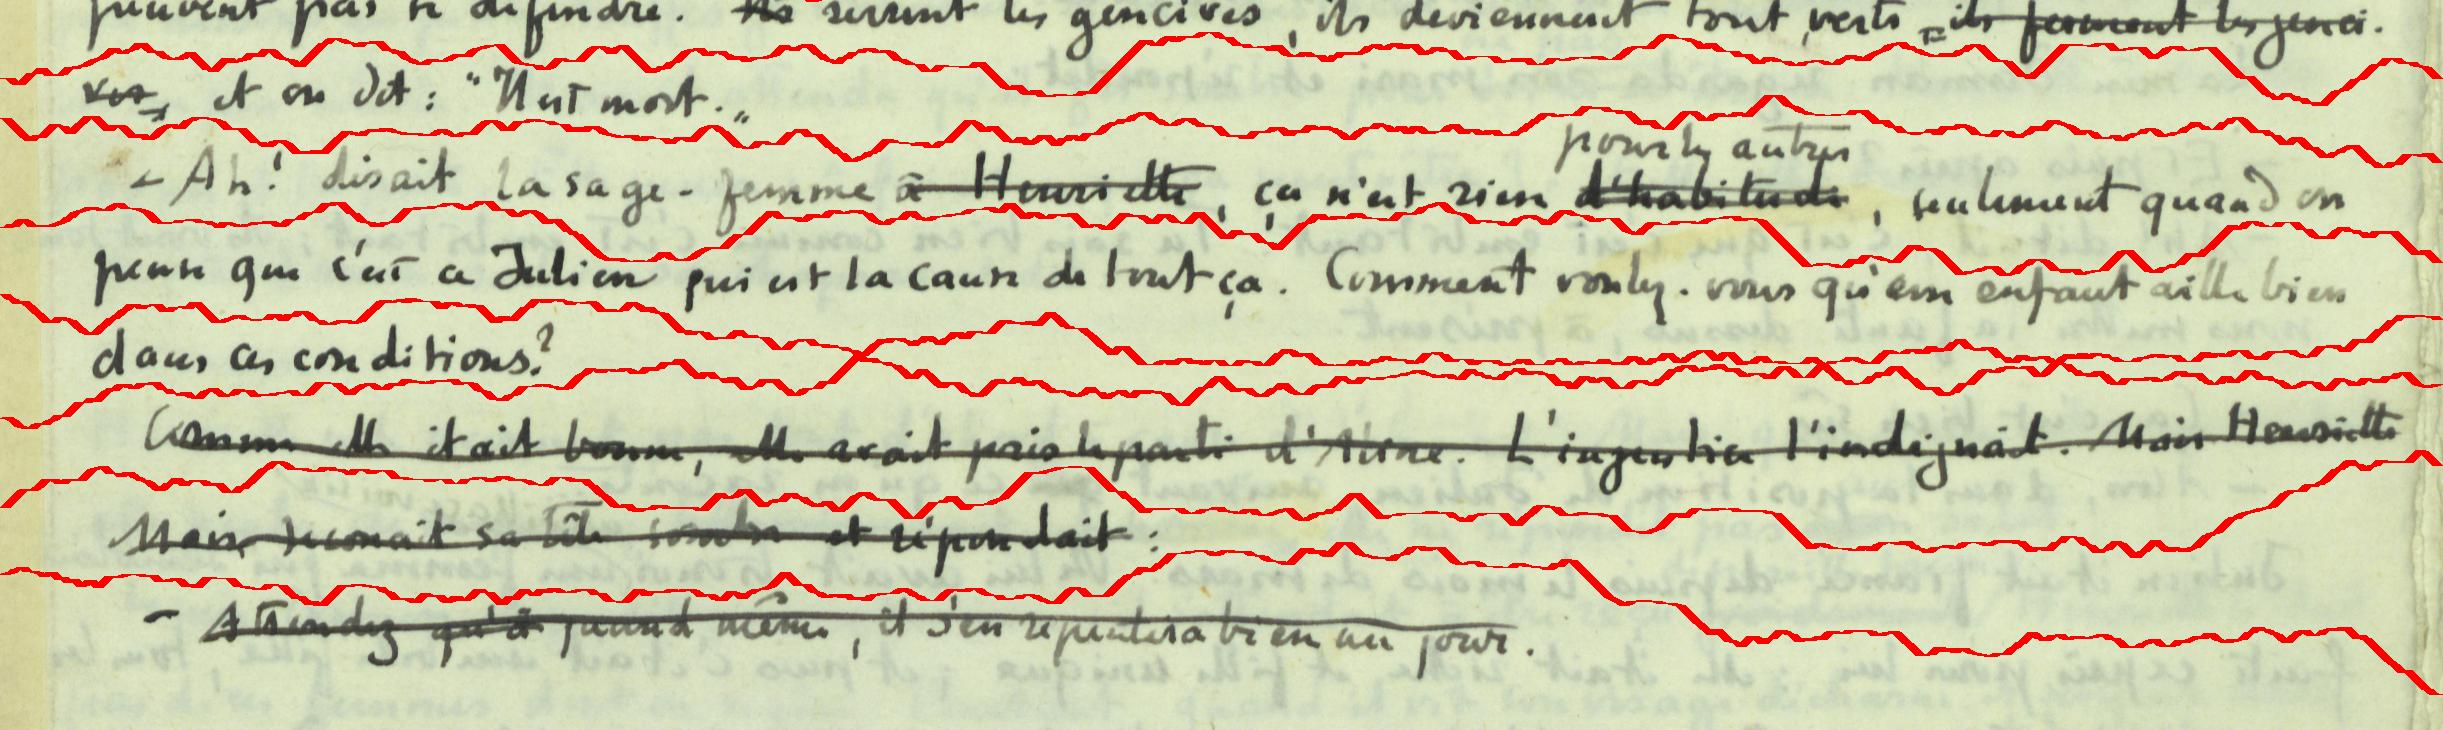
\includegraphics[width=\linewidth]{images/seams.jpg}
	\caption{Paths dividing a text block into lines. (from \cite[figure 5a]{arvanitopoulos2014seam})}
        \end{subfigure}
        \begin{subfigure}[t]{7cm}
        \centering
        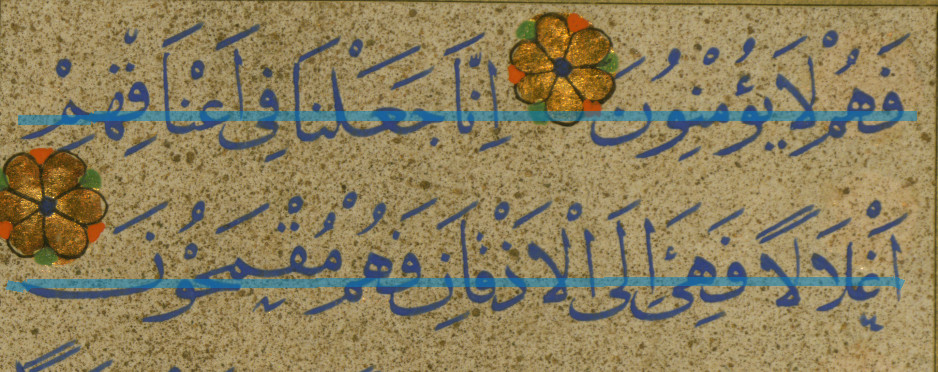
\includegraphics[width=\linewidth]{images/bl.jpg}
	\caption{Baselines (detail of Walters W.578 fol. 5a)}
        \end{subfigure}
        \begin{subfigure}[t]{7cm}
        \centering
        \includegraphics[width=\linewidth]{images/bbox.jpeg}
	\caption{Bounding box around a line (detail of Penn Libraries CAJS Rar Ms 132 fol. 53v)}
	\label{fig:intro_bbox}
        \end{subfigure}
	\caption{Principal representations of lines}
        \label{fig:intro_para}
\end{wrapfigure}

The prevalent paradigm since the development of segmentation-free text
transcription that is able to recognize a sequence of characters at once has
been text line segmentation. While the \emph{what} is evident, the
representation of the text lines is of more interest. The three principal
representations with spread in both research and practical applications are
paths, bounding boxes, and baselines (see figure~\ref{fig:intro_para}).
Axis-aligned bounding boxes, i.e. a bounding box whose edges are parallel to
the image boundary, which contains all the textual content of a particular line
and have an, often implicit, orientation are the most basic practical way to
encode a text line.  One of the benefits of this representation is that
rectangular boxes are a natural fit to the rectangular line strips ingested by
text line transcription methods, and therefore require only minimal processing
in the transcription method. There is a wide array of methods which fit
machine-printed and handwritten text to bounding boxes such as those described
in ~\cite{marti2001influence,papavassiliou2010handwritten} or the LA module in
the OCRopus system~\cite{Breuel03highperformance}. In general, these text line
segmenters struggle with slanted or curved texts, either natural or as a result
of the digitization process, and require the aforementioned preprocessing to
eliminate skew and warping but are inherently unable to accurately segment
multi-oriented and highly curved text. A minor extension implemented in the
Tesseract LA module which increases the versatility of the text line model is
to allow rotation of the text bounding box in combination with an explicit
orientation detection algorithm~\cite{smith2007overview}.

Paths are a flexible alternative which allow the segmentation of slanted and
curved lines with relative ease. They encode blocks of lines that are roughly
in the same orientation through a series of separating linear or non-linear
paths. This representation has one drawback: segmenting a page document into
blocks can already prove to be a challenge. Early methods utilized projection
profiles~\cite{antonacopoulos2004document}, at times piecewise to improve
segmentation of curvature~\cite{zahour2001arabic}. More recent approaches tend
to treat path finding as an optimization problem using the Viterbi
algorithm~\cite{tseng1999recognition} or seam carving~\cite{arvanitopoulos2014seam,zhang2014text}. Notwithstanding the fact that this
approach is superior to using bounding boxes to ensure tight bounds around
curved and/or slanted lines, the above-mentioned block segmentation challenge
prevented its dissemination, and it has never been implemented in any
mainstream OCR engine. It should be noted, however, that the
Aletheia~\cite{6065274} document analysis system implements human-triggered
path-based line segmentation.

Baselines are currently the state of the art for text line segmentation in
highly challenging historical documents. The baseline is an imaginary line
which letters rest on, although letters frequently have parts (called
descenders) that dip below it. It is a fairly common concept which exist in a
large number of alphabetic writing systems, although certain scripts (e.g.
Hebrew, Tibetan, or Bengali) are written with a hanging base or topline
instead, and most logographic scripts such as Chinese do not have any in the
strict typographic sense. In spite of these variations, approximations can
often be systematized well enough to allow the processing of most scripts using
a baseline LA method.

Representing text lines by their baseline has one major advantage: the model
can accommodate arbitrary curvature by defining the baseline as a simple
polyline, i.e. a sequence of straight line segments. Apart from being able to
express any text written in linear writing systems compactly, baseline
representation has the added benefit of allowing rectification through
projection of the individual polyline segments onto a straight line. However,
there is also one drawback. A baseline alone is not sufficient to extract a
complete text line as it is not known which points around it belong to the line
in question or to adjacent content. As a result, baselines are usually
accompanied with additional bounding polygons. Baseline representation appears
in the literature as early as 1989~\cite{srihari1989analysis}. However, it went
largely unnoticed until recently, except for a few segmentation systems~\cite{Breuel03highperformance,smith2007overview} that used baselines internally
for clustering line blobs. Two factors helped their popularization among
researchers. Firstly, \cite{romero2015influence} showed that bounding polygons
had only but a small impact on transcription error rates, although this
certainly does not hold true for all historical documents. Secondly,
\cite{diem2017cbad} published cBAD, a large dataset annotated with
(poly-)baseline, and an evaluation metric for a ICDAR contest. This was
followed by a larger and more complex dataset in 2019~\cite{diem_markus_2019_3568023}. Since then, the literature has produced a
number of methods
\cite{xu2018multi,quiros2018multi,mechi2019text,oliveira2018dhsegment,romain2019semi,gruning2019two,melnikov2020fast}.
They usually combine a deep neural semantic segmentation method (common choices
are U-Nets and FCNs) with a postprocessing heuristic of varying complexity.
While progress in accuracy levels using the ICDAR contest dataset have been
impressive, practical hurdles remain. Since bounding polygons are not part of
standard evaluation metric, they do not define an algorithm for computing one.
Likewise, the metric does not take line orientation into account and the cBAD
dataset is almost exclusively made of upright lines. As a result, there is
neither academic incentive nor any datasets available to develop baseline LA
methods that are able to determine line orientation effectively. Currently, two
OCR systems include trainable baseline LA systems: Transkribus and Kraken (see
chapter~\ref{ch:kraken}), to which must be added support in the eScriptorium
VRE and the OCR-D workflow engine, via the Kraken module.

Other text line representations do exist but they are rarely used in practice.
Pixel labelings and bounding polygons are relatively easy to produce using deep
convolutional ANNs for semantic \cite{pastor2016complete,alberti2019labeling}
or instance segmentation \cite{prusty2019indiscapes}. However, they require
tedious training data acquisition. In addition, in the case of semantic
segmentation-based methods, separation between close lines can be problematic.
Furthermore, without an additional way to determine line orientation or
estimate line curvature, text recognition on rotated and highly curved purely
polygon-bounded lines affects recognition accuracy negatively. This is due to
the fact that lines cannot be effectively normalized to the rectangular line
image strips processed by text transcription methods. 

Some ancillary tasks are also associated with layout analysis. Region
segmentation (also known as page segmentation or zoning) divides a document
image into semantic regions such as main text, decoration, illustration, \dots.
Its output has several applications: to improve the OCR engine’s final textual
output through semantic annotation; to restrict the range of valid output in
other tasks, e.g. by only providing regions of interest to the text line
detector or by limiting the text transcription method to numerals in a postal
code field; or to increase the information available to algorithms for reading
order determination. 

Region segmentation is well-established as a task. There are hundreds of
hand-crafted region segmentation algorithms. They are often optimized for
particular use cases and employ various filtering~\cite{PAVLIDIS1992484},
cutting~\cite{ha1995recursive,kruatrachue2005fast}, and
clustering~\cite{drivas1995page,kise1998segmentation} techniques. As for text
line segmentation, the capabilities of deep convolutional ANNs have made them a
popular choice, and since 2018 a number of publications have focused on this
task~\cite{wick2018fully,oliveira2018dhsegment,xu2018multi,quiros2018multi,he2017multi,chen2017convolutional,monnier2020docextractor}.
A number of systems such as \cite{oliveira2018dhsegment} (U-Net),
\cite{xu2018multi} (FCN), and \cite{quiros2018multi} (GAN with custom CNN) have
implemented an attractive proposition: the possibility to perform both baseline
detection and region segmentation with the same network architecture, or even
the same model \cite{quiros2018multi,xu2018multi}. Certain OCR engines have
started to incorporate neural region segmentation, for instance
anyOCR~\cite{bukhari2017anyocr}, Transkribus, or Kraken. Other systems (e.g.
Tesseract or OCR4all) retain heuristics for this purpose.

Reading order determination (ROD) is an integral part of layout analysis,
albeit it is often overlooked. While systems as described above detect layout
structure, they fail to give any information as per how layout elements are
related logically.  The reading order (i.e. the order in which human readers
will read textual and non-textual components) constitutes one of the most
important logical structures and is critical to understanding a document. It
may sound simple at first, as most modern documents are read following a simple
top-to-bottom order. However, there is a large body of documents for which this
is no trivial matter. Newspapers, for example, contain articles spanning
multiple columns and pages; scholarly editions have critical apparatus which do
not obey the normal reading order; and historical manuscripts often display
extensive marginal notes, interlinear additions, and parallel texts. The
literature on the topic is sparse, in particular when compared to many other
DIA tasks. As a matter of fact, the current state of the art has not evolved
since the early 2000s in any substantial way. \cite{nagy1984hierarchical,ishitani2003document,meunier2005optimized} generate
a region tree with X-Y cuts which is subsequently ordered using simple
heuristic rules (top-to-bottom, left-to-right). \cite{Gao} incorporates
language modelling to determine likely text block sequences in newspapers.
\cite{Breuel03highperformance} uses topological sorting to sort individual text
lines on a page. \cite{AielloIJDAR2002} utilize decision trees that incorporate
both spatial and linguistic features, so as to fit to a complex document
understanding model. A partially trainable system using linear programming to
reconcile user-defined constraints is proposed in \cite{malerba2008machine}.
Despite the fact that some of the above methods are indeed intended for highly
complex documents, all of them make assumptions regarding the spatial ordering
of lines which are ill-suited to many historical documents. However, graph
neural networks have shown promise in logical document structure
analysis~\cite{dejean2019versatile} and might be adapted for ROD in the future.

ROD implementations in OCR engines mirror the current state of the art in
research. OCRopus and Kraken use \cite{Breuel03highperformance}. Tesseract
employs a simple rule-based algorithm described in \cite{5277715}. The OCR-D
workflow engine does not treat ROD as a separate task, instead relying on the
implicit order provided through the respective LA modules.

\subsection{Transcription}

As described in section \ref{s:la}, conventional OCR systems were constructed
around character classifiers. Character classifiers require accurate character
segmentations, which are frequently difficult to obtain for historical,
degraded, and cursive text. To solve this problem, different segmentation-free
methods have been proposed. They recognize one sequence of characters (e.g. a
word or a line) at a time. It should be noted that if the term
segmentation-free is commonplace in the literature, it only applies to the
input data and the training process. This is due to the fact that it is often
possible to extract segmentation as well as estimates of character locations
from their output, as an implicit segmentation is performed internally.

It was via the adaptation of HMM-based methods used in speech recognition that
the earliest approaches, able to both perform sequential classification and to
produce an hypothesis for a possible segmentation, were designed
\cite{kaltenmeier1993sophisticated,rigoll1996comparison}. Such approaches can
be trained easily using Expectation Maximization. In addition, they allow
straightforward incorporation of domain knowledge such as language models, with
the goal of increasing their capacity to model long term dependencies. However,
most HMM OCR methods operate on feature representations that are calculated on
a sliding window over the text line, as is indeed necessary to reduce the
number of model parameters to avoid severe overfitting. HMM-based methods may
differ widely from one to another, in particular when it comes to the choice of
these types of features, and the literature abounds with descriptions of
different general-purpose and heuristic features. An outline of different
feature extractors, modeling granularity, and language models employed in
HMM-based OCR methods is contained in a 2009 survey~\cite{plotz2009markov}.

The inferiority of HMM-based methods to RNNs trained with CTC loss became
blatantly apparent in 2009, when a CTC trained multidimensional LSTM (MDLSTM)
\cite{graves2008offline} won three contests on French, Arabic, and Persian
handwriting transcription without any language-specific method adaptation.
Because the computational requirements of MDLSTMs for both inference and
training made them unsuitable to large scale applications, and also because
some doubts existed regarding their assumed superiority over
1D-LSTMs~\cite{puigcerver2017multidimensional}, simpler bidirectional LSTMs
(BiLSTM)~\cite{graves2008novel} became the basis for numerous derivations of
the general BiLSTM+CTC schema. The first hybrid convolutional and recurrent
neural network (CRNN) for natural scene text recognition was proposed in
\cite{shi2016end}. Meanwhile, \cite{dutta2018improving} augmented a basic CRNN
with a spatial transformer network block that learned to dewarp input text line
images. \cite{stuner2016cohort} incorporated lexicon verification to control a
cascade of text transcription RNNs. \cite{bluche2017gated} combined novel gated
convolutional layers with a multilayer BiLSTM and CTC loss. More complex
training procedures are sometimes constructed around these methods, for
instance incorporating auxiliary language model losses to adapt a transcription
model to an unseen language \cite{tensmeyer2018language}. Another example is
domain adaptation from synthetic machine-printed to handwritten text with
virtual adversarial training \cite{keret2019transductive}.

In recent years, various attempts were made to find alternatives to RNNs or CTC
for text transcription. Apart from the everlasting search for greater accuracy
and generalization, RNNs (and especially LSTMs) are slow and cannot be
parallelized easily. CTC has the aforementioned limitations, to which one must
add complexity, not to mention that fast implementations suffer from
restrictions such as maximum target sequence lengths. Attentional models such
as \cite{sueiras2018offline,michael2019evaluating,kang2018convolve} replace CTC
with conventional losses. In general, they consist of an encoder and a decoder,
where the encoder produces a feature map.  Through an attention mechanism
(which can be of different types, including content- and location-aware
attention), the decoder can weigh at each decoding step the relative importance
of the different parts of the feature map. The number of times the decoder runs
steps is arbitrary, and characters are output directly from the weighted feature map. It
follows that these methods hardly allow the character sequence to align with
the input image. This contrasts with HMMs and CTC-trained ANNs sharply.
\cite{coquenet2020recurrence} describes a recurrence-free, CTC-trained, gated
convolutional ANN which, if compared to CRNNs, achieves similar (albeit
slightly lower) character error rates. Focusing on the recognition of in-air
handwritten Chinese text, \cite{gan2020air} proposes a system that uses
increasingly strided 1D convolutional layers to achieve large receptive fields
in the feature extractor, quite similarly to non-causal temporal convolutional
networks (TCNs). While the complete ANN architecture includes some final LSTM
layers, an ablation study shows that the TCN on its own achieves error rates
that are similar to a simple two-layer LSTM.

As state-of-the-art hybrid CRNNs trained with CTC loss largely surpass older
HMM-based systems and have existed for a few years, many OCR engines include
(C)RNN+CTC transcription modules. The OCRopus system uses a one-layer
bidirectional LSTM trained with a particular variant of CTC loss, implemented
completely in Python. The latest (fourth) version of Tesseract includes a
dynamically configurable neural networking library which is highly optimized
for inference on CPU. In addition, Tesseract’s default network configurations
include unconventional summarizing LSTM layers that compute local features as
the last time step output of an LSTM layer ingesting a one-pixel-wide vertical
slice of the line, one pixel at a time. The OCR4All system uses the Calamari
text classifier, which implements an ensemble method of confidence-weighted
voting of cross-fold-trained CRNNs \cite{wick2018calamari}. Kraken implements a
configurable neural networking backend with a model specification
language~\ref{app:kraken}, defaulting to a simple six layer CRNN.
anyOCR~\cite{bukhari2017anyocr} uses BiLSTMs trained in a conventional
supervised fashion with CTC, but includes a procedure to harvest imprecise
training data through manually labelled character clusters. It aims to
drastically reduce training data requirements.

\subsubsection{Specialty tasks}

Certain specialty tasks exist without being part of any general-purpose OCR
systems. Either the material they are designed for is too uncommon and
dissimilar to writing systems for natural languages, or the state of the art is
not sufficiently accurate to warrant implementation in practical OCR engines.

Table analysis is a task in DIA whose goal is to detect and recognize both the
contents of a table and its logical structure. Despite a long history of
research in table processing methods which extends far into the early
nineteen-nineties \cite{zanibbi2004survey}, this task is still considered
unsolved even for modern printed tables \cite{gao2019icdar}. There is limited
research pertaining to the processing of historical tabular material. Even
hand-crafted methods that are optimized for a particular table style have high
error rates~\cite{lehenmeier2020layout}. Since table retrodigitization remains
an area of commercial interest in the data entry industry, certain proprietary
OCR engines (e.g. Abbyy FineReader) include table detection and structure
recognition.

Optical Music Recognition (OMR) aims to transcribe sheet music into a
ma\-chine-readable representation. The process is analogous to OCR in many ways;
yet the term OMR remains rather ill-defined. It encompasses output
representations (e.g. MIDI) that one would not traditionally associate with
OCR. In addition, musical notation behaves quite differently from most scripts
used for natural language, as it is a featural writing system whose information
is contained both in the ordered sequences of symbols and their spatial
relationships. Some researchers such as \cite{calvo2020understanding} reject
the categorization of OMR as a sub-type of OCR or \emph{OCR for music} and the
field has developed a number of OMR-specific tasks such as staff processing and
musical information reconstruction that have no equivalent in the domain of OCR
(see \cite{shatri2020optical} for a recent survey of OMR tasks and methods).
For practical purposes, the OCR and OMR research fields are distinct. OCR
engines are not capable of processing musical notation and vice-versa.

Likewise, digital map processing is usually treated separately even when the
goal is limited to textual content extraction. This is due to the fact that
non-text elements make up for a larger proportion of the total writing surface
than most other documents. This makes text finding harder for most LA methods.
However, it should be noted that in comparison to other DIA applications text
transcription in maps can better exploit domain knowledge, as the nature of
naturally-expressed geographical data allows alignment with other maps and
incorporation of toponym
dictionaries~\cite{weinman2013toponym,weinman17geographic,sun2020aligning}.
Complete map understanding requires not only text line detection and region
segmentation layout analysis but also the extraction of cartographic features
such as map symbols and contour lines. Most text LA systems are ill-suited for
this purpose, and it is therefore generally performed using dedicated
segmentation methods such as \cite{uhl2018spatialising,liu2020superpixel}.

\subsection{Virtual Research Environments for DIA, OCR, and Digital Humanities}

Virtual Research Environments encompass a broad range of research support
systems that share common characteristics. They offer a web-based working
environment and are tailored to serve the needs of a \emph{community of
practice} \footnote{Communities of practice as defined in
\cite{wenger1999communities} are individuals that are united in action and in
the meaning that an activity has for them as individuals and as a collective,
i.e. communities are composed of active practitioners who create a community
through self-identification with and exchange on a particular, in our case
scholarly, activity.}. They provide a comprehensive catalogue of tools to
support the targeted community in accomplishing its goals. They are open and
flexible with respect to service offering and lifetime, and promote controlled
sharing of both intermediate and final research results by guaranteeing
ownership, provenance and attribution\cite{candela2013virtual}. They are not
specific to OCR or the humanities and can be designed around all kinds of
research activity.

A number of web-based platforms offer manual or computer-assisted segmentation,
transcription, and recognition for certain categories of material in the
humanities field. However, whether they can be considered actual VREs is open
to question. Most platforms are developed within particular institutional
frameworks as project-specific tools, without active buy-in from practitioners
falling outside well-defined collaborations. This situation explains the lack
of platforms that satisfy all criteria for VREs. In this review, we will relax
the criteria while still limiting our review to tools whose functionalities at
least partially overlap with eScriptorium’s.

Most platforms implement specific methods to suit the needs of a particular
scientific project, and most research projects are of relatively short duration
and seek to solve specific research questions. As a result, in typical settings
dedicated platforms are not concerned with implementing a complete catalogue of
methods to perform an activity fully. They also rarely create a scholarly
community around them, albeit they can be considered as being part of a fabric
of loosely-coupled tools that could be made to interoperate through common data
interchange formats. Crowdsourcing applications for transcription of historical
documents have proved to be a particularly successful type of platforms. Tools
like the Bentham Transcription Desk~\cite{moyle2011manuscript} discard any
automatic processing to retain simplicity in implementation. Such platforms are
rarely openly accessible. In other words, data on which users can perform
activities is predetermined by the platform’s operators; imports are often
already processed extensively through external means. The TypeWright OCR
correction and digital edition creation tool~\cite{typewright} is a good example
of this. The only raw OCR data that it makes available was created by the eMOP
project's internal pipeline. On the other hand, it should be noted that a
fairly large number of platforms accepting the use of arbitrary data do exist.
They are, however, of very limited capability. For instance, \cite{webaletheia}
is a platform whose purpose is to create segmentation ground truth data with
some low-level computer vision assistance. Another example is the
HInDoLA~\cite{trivedi2019hindola} platform, which is solely intended to aid the
layout analysis of palm leafs. LAREX~\cite{reul2017larex} is a semi-automatic
tool for layout analysis of early printed books. It can be interfaced to
external OCR tools through data exports in PageXML format. PoCoTo
~\cite{vobl2014pocoto} is a web service geared towards the postcorrection of OCR
output with language modelling assistance.

When it comes to communities of OCR practitioners in the humanities, the
Transkribus~\cite{kahle2017transkribus} platform comes closest in meeting the
VRE definition. It was designed as a comprehensive platform for computer-aided
layout analysis, transcription and information retrieval. It offers all the
basic tools necessary to the average scholar interested in retrodigitization of
historical handwritten and printed material. Unfortunately, the closed nature
of the platform hampers interested scholars’s capacity to share their work
while being guaranteed ownership of their work. While data can be imported and
exported in standard formats freely, artifacts trained in specific OCR tasks
(i.e. layout analysis and transcription models) with user-created data are
locked inside the platform. Added to the platform’s recently adopted pricing
model, it presents not only a significant deficit of ownership but also a
barrier to the reproducibility of results.

While eScriptorium is not yet feature complete and access to the platform of
the public is currently limited, albeit the source code of all components is
publicly available and a number of instances are set up at different research
groups and institution, it already fulfills the VRE definition. It supports the
full gamut of OCR functions needed for the processing of historical material,
permits users to selectively share the product of their work, and provides
interfaces to import and export all data and workflow-produced artifacts.

\printbibliography[heading=subbibliography]
\endrefsection
